% vim: set tabstop=4 :
%**********************************************************
%\chapter{提案手法にあたる章}
%\chapter{格子分割を用いた進行方向計算の削減手法}
\chapter{格子分割による進行方向ベクトル計算の削減手法}
\label{sec:method}
%**********************************************************
SFMの運動方程式は,エージェントの位置が変わるたびに,
目的地までのベクトルを表す$e$や周囲のエージェントを避ける力$f_{ij}$,
障害物を避ける力$f_{iW}$の再計算が必要となる.
周囲のエージェントを避ける力$f_{ij}$の計算は,時間ステップごとにすべての
エージェントの位置が変化するため,解析中のみに計算が可能である.
一方,ベクトル$e$や障害物を避ける力$f_{iW}$は,エージェントの位置に
応じて決定し,壁や机などの障害物の座標が固定であることから,解析前に計算が可能である.

そこで,本論文では,格子状に分割した領域ごとにベクトル$e$と障害物を避ける力$f_{iW}$を
あらかじめ計算することで,解析中の進行方向の再計算を削減する.

\section{格子分割を用いた進行方向計算手法}
本手法は,解析領域を格子状に分割し,格子ごとに進行方向ベクトル$e$や
障害物を避ける力$f_{iW}$をあらかじめ計算する.
進行方向ベクトル$e$は,式\eqref{eq:sfm_siki1}に示すSFMの運動方程式から
$v_i^0(t)$が係数である.一方で,障害物から受ける力$f_{iW}$は,
式\eqref{eq:sfm_siki1}に示すように,式の第3項である.
このため,進行方向ベクトル$e$と障害物を避ける力$f_{iW}$は,
別々の配列に格納する必要がある.
\figref{fig:5_teian_flow1}に格子分割を用いた
進行方向ベクトル計算の削減手法のフローチャートを示す.
\figref{fig:5_teian_flow1}中の前処理は,提案手法に必要である格子ごとの進行方向や
壁を避ける力を算出する.
\figref{fig:5_teian_flow1}中の運動方程式を用いた計算は,
エージェントの進行方向を計算する処理であり,
エージェントの進行方向ベクトル$e$や
障害物を避ける力$f_{iW}$を前処理で算出した値を参照する.

\figtb{提案手法の解析全体のフローチャート}{}{4.5}{5_teian_flow1.eps}{5_teian_flow1}

%\subsection{格子分割を用いた進行方向ベクトル$e$の計算方法}
\subsection{格子ごとの進行方向ベクトル$e$の計算方法}
進行方向ベクトル$e$は,目的地に進むベクトルであり,エージェントの座標から
目的地の座標までのベクトルである.
このため,ベクトル$e$は解析領域を格子状に分割した領域ごとの中心座標から
目的地の座標までのベクトルを計算することで,解析前に計算が可能となる.
\figref{fig:grid_ex1}に格子分割した進行方向の例を示す.
%
\figtb{提案する格子分割の例}{}{9}{ex1.eps}{grid_ex1}
%
\figref{fig:grid_ex1}中の○はエージェントであり,エージェントA,Bが1つの目的地に向かう
様子である.
図中のエージェントBは,エージェントAの位置に移動したとき,エージェントAと同じ進行方向に
なる.
このため,解析領域を分割し,格子ごとに進行方向を算出することで,解析中の
進行方向の再計算が削減できる.
目的地と障害物が含まれる格子は,エージェントが正しく目的地に進むようにするために,
0ベクトルを格納する.
0ベクトルが格納された格子中に存在するエージェントは,
改めて個別に進行方向ベクトル$e$を計算する.
格子ごとの進行方向は,格子の中心座標から目的地までのベクトル$e$を求め,配列に格納する.
目的地の他に経由地が複数存在する場合,進行方向は,経由地ごとに異なるため,経由地ごとに違う配列に格納する必要がある.
\figref{fig:ex2}に経由地が複数存在する例を示す.
\figref{fig:ex2}中の右図は経由地の進行方向,左図は目的地の進行方向,青色の矢印は経由地に進む進行方向,
青矢印は目的地の進行方向,0は進行方向を個別計算するための0ベクトル,オレンジ色の四角は机などの障害物を示す.
\textbf{(要工事:元となる画像がない)}
\figref{fig:ex2}のように,経由地と目的地の進行方向は,それぞれの座標が異なるため,ベクトル$e$も大きく異なることから,
それぞれ別の配列で保持する必要がある.
式\eqref{eq:route_youso_size}に進行方向ベクトル$e$を格納するための配列の要素数を算出する式を示す.
%
\begin{eqnarray}
 \mbox{進行方向の格子の要素数[個]} = 
 \big( \frac{\mbox{解析領域[m]}}{\mbox{格子サイズ[m]}} \big) ^ 2 \times  2 \times \mbox{経由地数[個]}
 \label{eq:route_youso_size}
\end{eqnarray}
%
式\eqref{eq:route_youso_size}のように,進行方向を格納する配列は,
解析領域の大きさや格子サイズの小ささ,経由地数の大きさに応じて
要素数が増加する.
また,進行方向を格納する配列の前処理にかかる時間は,
配列の要素数に応じて格子ごとの進行方向計算回数が増加するため,
配列の大きさに応じて増加する.

%\figtb{経由地がある配置の例}{}{3}{5_original_ex.eps}{5_origin}

%\figtb{経由地がある場合の進行方向の例}{}{7}{ex2.eps}{ex2}
\figtb{経由地がある場合の進行方向の例}{}{12}{5_e_vec_ex.eps}{ex2}
%\figtb{シミュレーション中の進行方向計算のフローチャート}{}{8.5}{5_e_flow.eps}{5_e_flow}

%\subsection{格子分割を用いた障害物を避ける力$F_{iW}$の計算方法}
\subsection{格子ごとの障害物を避ける力$F_{iW}$の計算方法}
障害物を避ける力$F_{iW}$は,エージェントの座標と障害物の座標に応じて変化する.
障害物は,机や壁などの固定された物であるため,座標が変化しない.
このため,障害物を避ける力$F_{iW}$は,解析領域を格子状に分割した領域ごとの
中心座標と障害物の座標から解析前にあらかじめ計算が可能となる.
\figref{fig:preparation_fiw}に格子分割した障害物を避ける力$F_{iW}$を示す.
\figref{fig:preparation_fiw}中の四角は解析領域を格子状に分割した格子,
黒点は格子の中心点,緑色の丸は格子の中心点からの影響範囲,オレンジ色の
丸は壁粒子,赤色の矢印は黒点の中心点が受ける障害物を避ける力$f_{iW}$である.
\figref{fig:preparation_fiw}の例は,黒点が存在する格子が受ける障害物を避ける力$f_{iW}$
を示しており,黒点の中心点から緑色の範囲に存在する壁粒子から力を受ける.
各格子は,\figref{fig:preparation_fiw}のように格子の中心点の座標を
用いて障害物を避ける力を計算する.
壁を避ける力$F_{iw}$を格納する配列は,
経由地が変わっても変化しないため,解析領域全体で一つとなる.
式\eqref{eq:fiw_youso_size}に障害物を避ける力$F_{iW}$を格納する配列の要素数を示す.
%
\begin{eqnarray}
 \mbox{障害物を避ける力を格納する格子の要素数[個]} =  \Big( \frac{\mbox{解析領域[m]}}{\mbox{格子サイズ[m]}} \Big) ^ 2 \times 2
 \label{eq:fiw_youso_size}
\end{eqnarray}
%
式\eqref{eq:fiw_youso_size}に示すように,障害物を避ける力を格納する配列の要素数は,
解析領域と格子サイズに応じて決まり,解析領域を格子サイズで割った値の二乗が配列の要素数となり,
障害物を避ける力$F_{iW}$がxとy方向に存在するため,要素を2倍した値が障害物を避ける力$F_{iW}$を
格納する配列の総要素数になる.
\figref{fig:5_teian_flow2}に格子分割を用いた進行方向の計算回数削減手法の前処理のフローチャート
を示す.
\figref{fig:5_teian_flow2}中の$F_{iW}$配列は障害物を避ける力$F_{iW}$を格納する配列,
進行方向配列は進行方向ベクトル$e$を格納する配列,
$F_{iW}$のxインデックスとyインデックスは$F_{iW}$配列に格納するためのインデックスであり,
すべての要素に値を格納するためのループである.
同様に,進行方向配列のxインデックスとyインデックスは進行方向ベクトル$e$を配列に格納するための
インデックスであり,すべての要素に値を格納するためのループである.
進行方向ベクトル$e$は,経由地ごとに異なるため,経由地数分のループが前処理に必要となる.

%障害物が含まれる格子と周辺の格子に0を入れることを書く.

\figtb{格子分割した障害物を避ける力$F_{iW}$の例}{}{10}{5_fiw_grid.eps}{preparation_fiw}

%\figtb{提案手法の前処理のフローチャート}{}{5}{5_teian_flow2.eps}{5_teian_flow2}

\begin{figure}[p]
 \begin{center}
  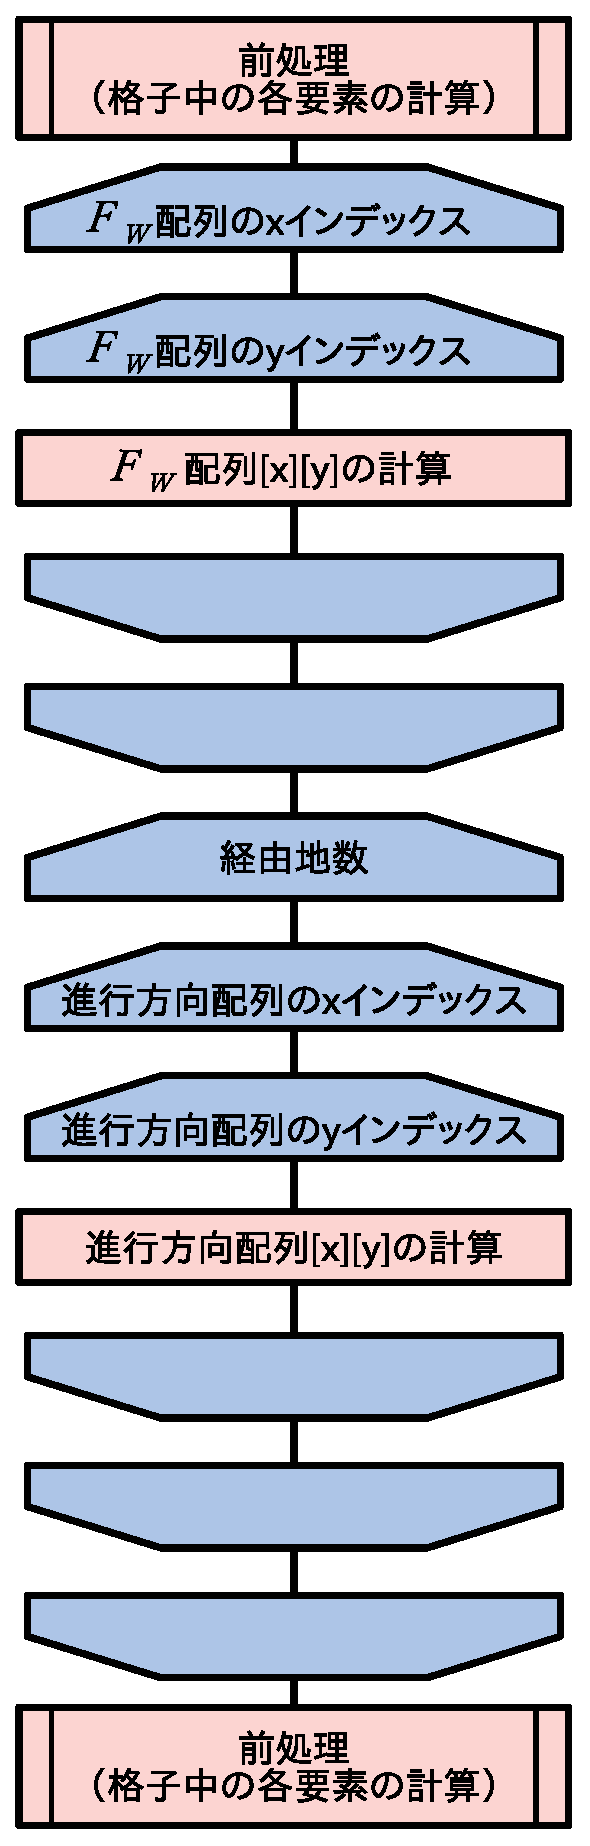
\includegraphics[width=4.5cm,clip]{figure/5_teian_flow2.eps}
  \caption{格子分割の前処理のフローチャート}
  \label{fig:5_teian_flow2}
 \end{center}
\end{figure}

\clearpage
\subsection{個別に進行方向を計算する格子の判定}
格子分割を用いた進行方向の計算回数削減手法は,精度の大幅な低下を防ぐために,
\figref{fig:ex2}のように目的地や障害物が含まれる格子とその周辺の格子に存在するエージェントを
個別に進行方向を計算するように設定する.
個別に進行方向する格子には,xとyの両方のベクトルに0が格納されているため,
解析中にエージェントが存在する格子に0ベクトルが格納されているか判定が必要となる.
\figref{fig:5_teian_flow2}に進行方向ベクトル$e$および障害物を避ける力$F_{iW}$の
解析中に個別計算するかどうかの判定のフローチャートを示す.
\figref{fig:5_teian_flow2}が示すフローチャートは,\figref{fig:5_teian_flow1}中の
解析中の運動方程式を用いた計算であり,エージェントの進行方向を求めるための計算である.
\figref{fig:5_teian_flow2}中の$F_{iW}$配列は障害物を避ける力$F_{iW}$を格納する配列,
進行方向配列は進行方向ベクトル$e$を格納する配列である.
\figref{fig:5_teian_flow2}に示すように,格子分割を用いた進行方向の計算回数削減手法は,
エージェントの座標から参照する配列の要素を求め,0ベクトルが格納されていない場合に
配列中の値を参照し,0ベクトルが格納されている場合に個別計算を行うことで解析中の
計算回数を削減する.

\figtb{提案手法の運動方程式計算のフローチャート}{}{9}{5_teian_flow3.eps}{5_teian_flow2}

\clearpage

\figtb{格子の進行方向とエージェントの進行方向で誤差が出る場合}{}{14}{5_kobetu_ex.eps}{5_kobetu_ex}
\figtb{近傍格子を個別計算の格子に設定する例}{}{8}{5_kobetu_ex1.eps}{5_kobetu_ex1}

\subsection{進行方向を個別に計算する格子}
提案手法は,\figref{fig:ex2}のように格子ごとに中心座標から目的地や経由地までの進行方向を決定するため,
格子が大きくなるほど,エージェントの進行方向と格子の進行方向で誤差が生じる.
\figref{fig:5_kobetu_ex}にエージェントの進行方向と格子の進行方向で誤差が生じる例を示す.
\figref{fig:5_kobetu_ex}中の緑色の四角は解析領域の緑色の範囲を拡大したもの,
右側の目的地の進行方向は\figref{fig:grid_ex1}の目的地の進行方向,
赤色のひし形は目的地,赤色の矢印は進行方向,
白色の丸はエージェント,青色の矢印は既存手法で求めたエージェントの進行方向である.
\figref{fig:5_kobetu_ex}のように,提案手法を用いた進行方向は,格子ごとの中心座標から
目的地の座標に向かうベクトルを算出するため,図中の赤色の矢印のように表せる.
一方で,SFMの運動方程式を用いて計算したエージェントの進行方向は,
エージェントの座標から目的地の座標に向かうベクトルであるため,
図中の青色の矢印のように表せる.
\figref{fig:5_kobetu_ex}中のエージェントは,格子のサイズが大きいことや格子の端にいるために,
本来の進行方向と大きく誤差が生じることがわかる.
このため,本提案手法は,個別に進行方向を計算する格子の設定方法を目的地や障害物が存在する
格子と近傍の格子にすることで,エージェントの進行方向に大きな誤差が生じないように対策する.
\figref{fig:5_kobetu_ex1}に近傍の格子を個別計算の格子に設定する例を示す.
\figref{fig:5_kobetu_ex1}中の左側の四角は解析領域を示しており,
左の四角は格子ごとの目的地に向かう進行方向,格子内の0は,個別でエージェントの進行方向を計算する格子である.
\figref{fig:5_kobetu_ex1}のように,提案手法は,目的地や障害物を含む格子とその近傍の格子を
個別計算することで,\figref{fig:5_kobetu_ex}のようなエージェントの進行方向の誤差が発生することを防ぐ.



%\figtb{シミュレーション中の$f_{iW}$計算のフローチャート}{}{8.5}{5_e_flow.eps}{5_e_flow}


\clearpage
\section{評価}
SFMを用いた人流シミュレーションに対する
格子分割を用いた進行方向の計算回数削減手法の有効性を確認するために,
既存手法であるセル分割法と提案手法を用いて人流シミュレーション
評価環境は,\tabref{tb:result_env}に示すマシンである.
本評価では,\tabref{tb:result_para}に示すパラメータを用いて
SFMの運動方程式を計算する.
本評価では,避難時のシミュレーションを再現するために,
エージェント数よりも壁粒子が多い配置にエージェントを一方向に進むような解析を行う.
\figref{fig:5_initialconf}に本評価に用いるエージェントの初期配置を示す.
\figref{fig:5_initialconf}中の黄色の四角は障害物(壁),赤色のひし形は目的地,
緑色の四角はエージェントの初期配置位置である.
\figref{fig:5_initialconf}のエージェントは,緑色の範囲内から赤色の目的地まで
進むように設定する.本評価では,格子サイズごとの計算回数の削減率や,解析時間の
有効性を評価するために,\figref{fig:5_initialconf}に示す配置の壁の間隔や粒子数を変えた
複数パターンを用いる.
\figref{fig:haba2}と\figref{fig:haba5},\figref{fig:haba10},\figref{fig:haba20}に
評価で用いる\figref{fig:5_initialconf}のエージェントの初期配置の壁間隔を変えた配置を示す.
また,\figref{fig:haba2_2},\figref{fig:haba2_3}に通路幅2mのときの配置(\figref{fig:haba2})
の壁粒子をそれぞれ2倍,3倍にした配置を示す.
図中の黒丸は壁粒子,紫色の丸はエージェント,青色の丸は目的地である.
図に示す配置のエージェントは40人,壁粒子は592個,経由地は1個,
解析領域は$50m \times 50m$である.
また,壁粒子を変えた配置(\figref{fig:haba2_2},\figref{fig:haba2_3})の
壁粒子数は\tabref{tb:haba_atusa}に示す通りである.
図中のすべてのエージェントは,青色の丸が示す目的地に向かうように設定する.
測定する格子サイズは,解析領域の一辺(50m)を半分ずつ割った値を用いる.

\begin{table}[t]
  \begin{center}
    \caption{評価環境}
      \label{tb:result_env}
      \begin{tabular}{c|c}
      \hline \hline
      CPU              & Intel Xeon CPU E5-2667w v2 \\ \hline
      メモリ           & 32GB                       \\ \hline
      OS               & Linux 6.5.8               \\ \hline
      コンパイラ       & gcc 13.2.0                  \\ \hline
      最適化オプション & -O3                        \\ \hline
    \end{tabular}
  \end{center}
\end{table}

\begin{table}[t]
  \begin{center}
    \caption{測定条件}
    \label{tb:result_para}
    \begin{tabular}{c|c}
      \hline \hline
      $A_i$            & 2000N                              \\ \hline 
      $B_i$            & 0.08m                              \\ \hline 
      $k$              & $1.2 \times 10^5 kg s^{-2} $       \\ \hline 
      $\kappa$         & $2.4 \times 10^5 kg m^{-1} s^{-2}$ \\ \hline 
      $v_i^0$          & $1.4$m/s                           \\ \hline 
      $m_i$            & $80$kg                             \\ \hline 
      $\tau_i$         & 0.5                               \\ \hline 
      $r_i$            & $0.25$m                            \\ \hline 
      相互作用範囲     & $5$m                              \\ \hline 
    \end{tabular}
  \end{center}
\end{table}


\begin{table}
  \begin{center}
    \caption{壁の厚さを変えたときの初期配置のパラメータ}
    \label{tb:haba_atusa}
    \begin{tabular}{c|c|c|c}
      \hline \hline
            & 壁粒子数[個] & エージェント数[人] & 経由地数[個] \\ \hline
      厚さ1倍 & 592  & 40 & 1 \\ \hline
      厚さ2倍 & 1184 & 40 & 1 \\ \hline
      厚さ3倍 & 1776 & 40 & 1 \\ \hline
    \end{tabular}
  \end{center}
\end{table}


\figtb{エージェントの初期配置}{}{11}{5_initialconfiguration.eps}{5_initialconf}

\clearpage

\dfig{通路幅2mの初期配置}{20231023_haba2}{haba2}{通路幅5mの初期配置}{20231023_haba5}{haba5}

\dfig{通路幅10mの初期配置}{20231023_haba10}{haba10}{通路幅20mの初期配置}{20231023_haba20}{haba20}

\dfig{通路幅2m(壁粒子数2倍)の初期配置}{haba2_2}{haba2_2}{通路幅2m(壁粒子数3倍)の初期配置}{haba2_3}{haba2_3}

\clearpage


%result figure {{{
\begin{figure}[tb]
	\begin{minipage}[b]{0.48\columnwidth}
		\begin{center}
		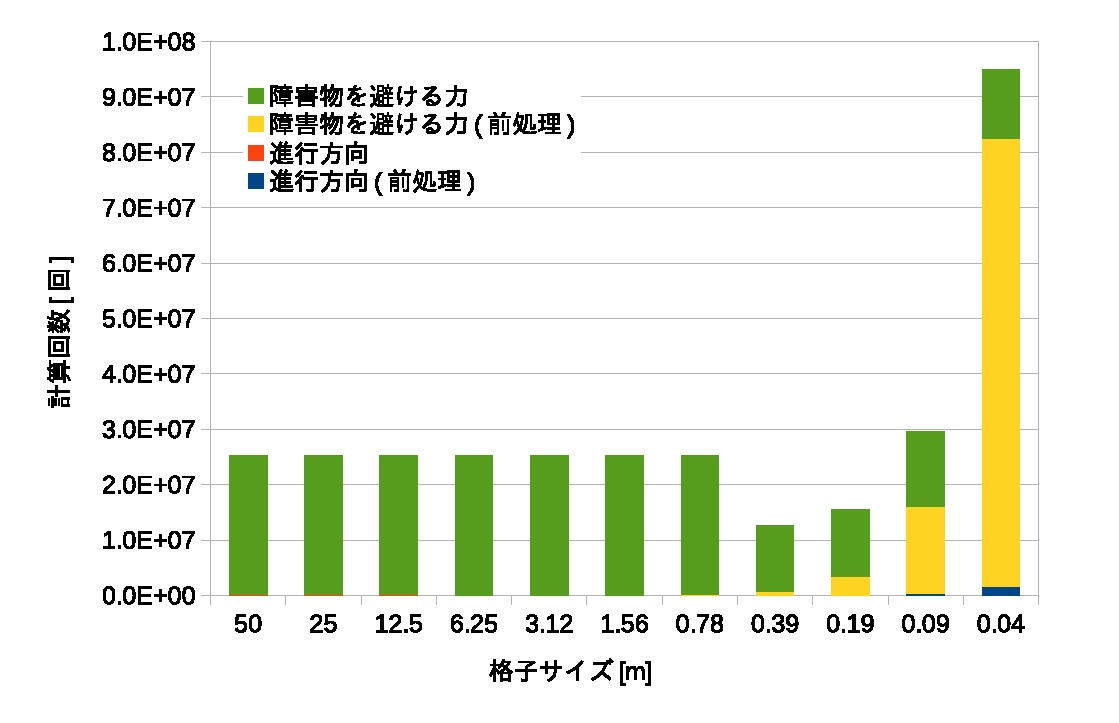
\includegraphics[width=\columnwidth]{figure/5_result_2m_times.eps}
		\caption{通路幅2mの格子サイズごとの計算回数}
		\label{fig:result_2m_times}
		\end{center}
	\end{minipage}
	\hspace{0.04\columnwidth}
	\begin{minipage}[b]{0.48\columnwidth}
		\begin{center}
		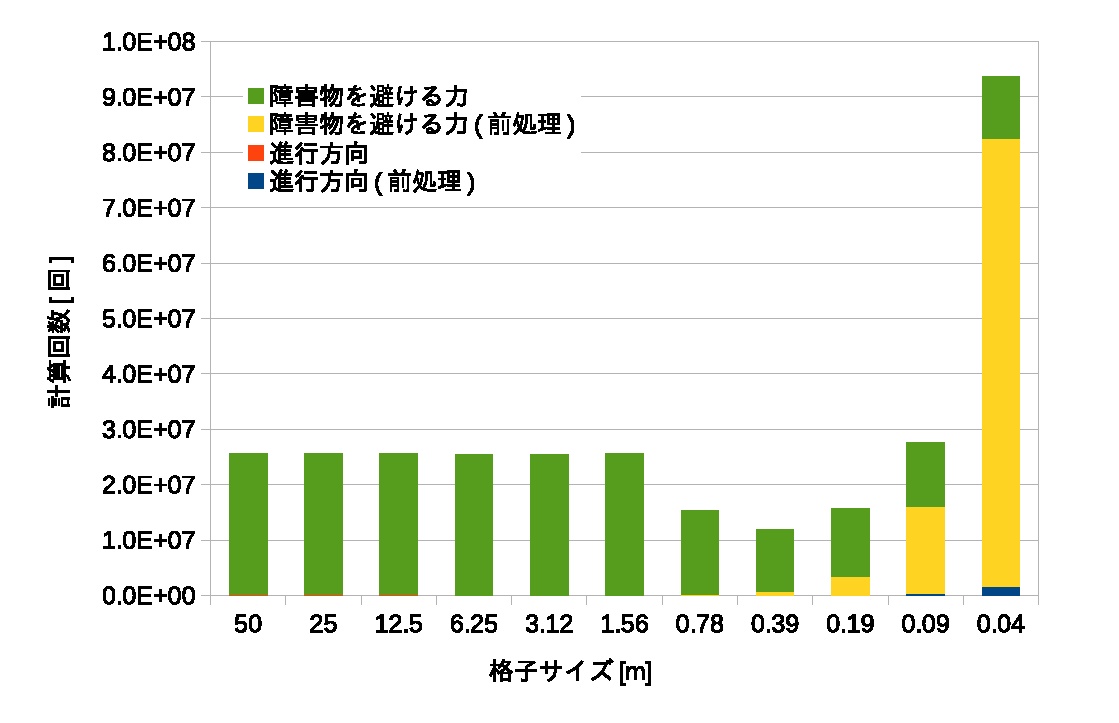
\includegraphics[width=\columnwidth]{figure/5_result_5m_times.eps}
		\caption{通路幅5mの格子サイズごとの計算回数}
		\label{fig:result_5m_times}
		\end{center}
	\end{minipage}
\end{figure}
%}}}
%result figure {{{
\begin{figure}[tb]
	\begin{minipage}[b]{0.48\columnwidth}
		\begin{center}
		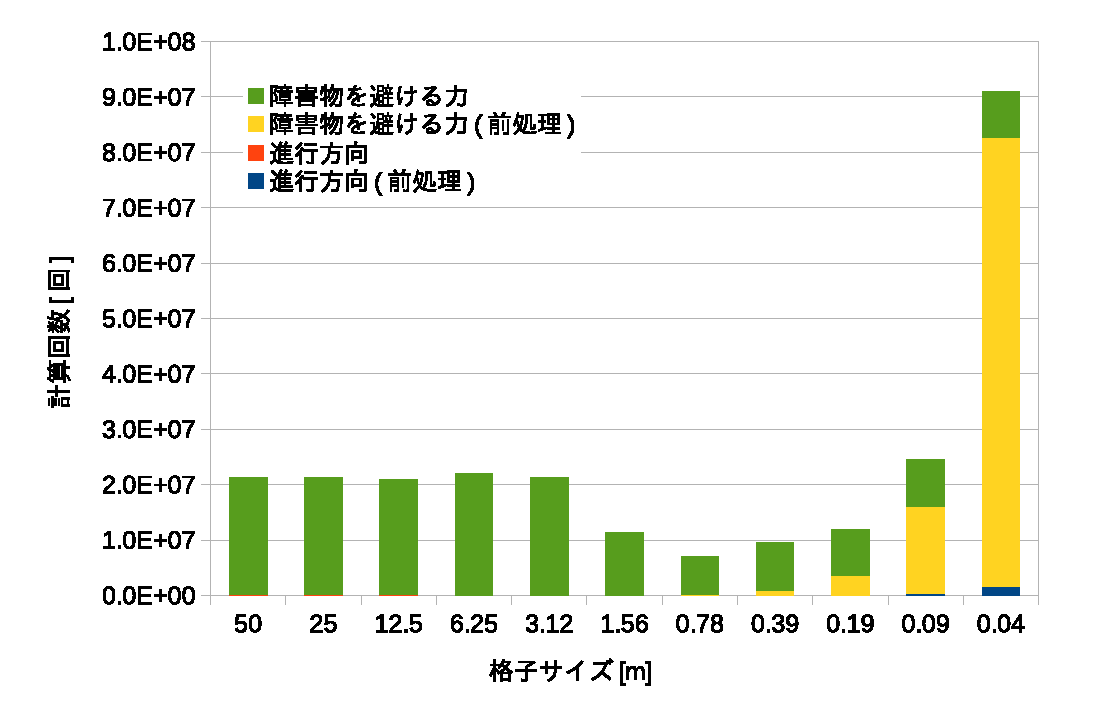
\includegraphics[width=\columnwidth]{figure/5_result_10m_times.eps}
		\caption{通路幅10mの格子サイズごとの計算回数}
		\label{fig:result_10m_times}
		\end{center}
	\end{minipage}
	\hspace{0.04\columnwidth}
	\begin{minipage}[b]{0.48\columnwidth}
		\begin{center}
		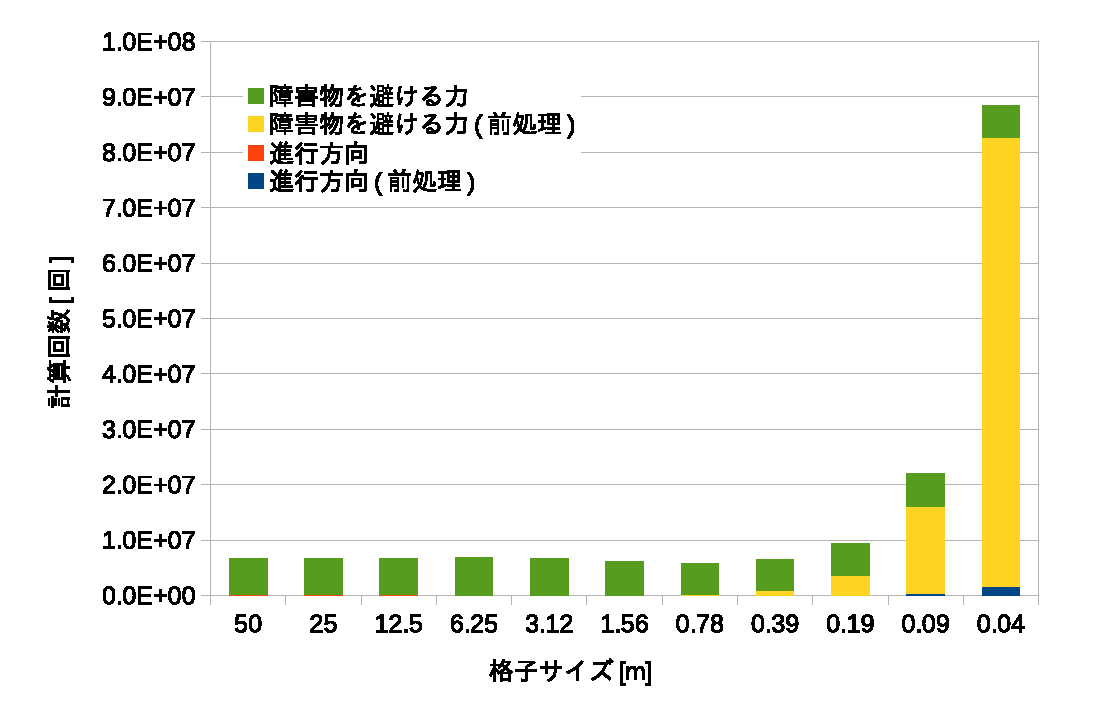
\includegraphics[width=\columnwidth]{figure/5_result_20m_times.eps}
		\caption{通路幅20mの格子サイズごとの計算回数}
		\label{fig:result_20m_times}
		\end{center}
	\end{minipage}
\end{figure}
%}}}

%削減率の表{{{
\begin{table}[tb]
  \centering
  \caption{各通路幅の格子サイズごとの計算回数の削減率[\%]}
  \label{tb:5_times_sakugenritu}
    \begin{tabular}{r|r|r|r|r}
    \hline \hline
              & 通路幅2m       & 通路幅5m       & 通路幅10m      & 通路幅20m     \\ \hline
        50.00 & 0.00           & 0.00           & 0.00           & 0.00          \\ \hline
        25.00 & 0.00           & 0.00           & 0.00           & 0.00          \\ \hline
        12.50 & 0.08           & 0.07           & 1.03           & 0.03          \\ \hline
        6.25  & 0.23           & 0.25           & -3.04          & -0.93         \\ \hline
        3.12  & 0.15           & 0.22           & -0.12          & 1.57          \\ \hline
        1.56  & 0.19           & 0.10           & 37.69          & 6.44          \\ \hline
        0.78  & 0.50           & 33.86          & \textbf{54.81} & \textbf{8.25} \\ \hline
        0.39  & \textbf{43.85} & \textbf{45.48} & 44.98          & 1.60          \\ \hline
        0.19  & 34.61          & 32.68          & 35.66          & -23.33        \\ \hline
        0.09  & -13.93         & -6.88          & -12.48         & -137.22       \\ \hline
        0.04  & -235.83        & -225.08        & -267.49        & -738.82       \\ \hline
    \end{tabular}
\end{table}
%}}}

\subsection{進行方向計算の計算回数}
\label{sec:5_calc_times}
本測定では,格子分割を用いた進行方向の計算回数削減手法の
有効性を評価するために,既存手法であるセル分割法と
格子分割を用いた進行方向の計算回数削減手法の計算回数を測定する.
測定する計算は,エージェントの進行方向の決定に必要な
エージェントの進行方向ベクトル$e$と
障害物を避ける力$F_{iW}$であり,前処理と解析中の回数である.
\figref{fig:result_2m_times},\figref{fig:result_5m_times},
\figref{fig:result_10m_times},\figref{fig:result_20m_times}に
各配置における計算回数を示す.
また,\tabref{tb:5_times_sakugenritu}に各配置における削減率を示す.
\tabref{tb:5_times_sakugenritu}に示す削減率は,式\eqref{eq:5_sakugenritu}
のように,セル分割法の各計算の総和$C_e$と提案手法の各計算の総和$C_p$を
用いて算出する.
%
\begin{eqnarray}
\mbox{削減率[\%]} = \Big ( 1 - \frac{C_p}{C_e}  \Big) \times 100
\label{eq:5_sakugenritu}
\end{eqnarray}
%

\figref{fig:result_2m_times}から\figref{fig:result_20m_times}より,
提案手法は,セル分割法よりも進行方向の計算回数が削減できる格子サイズが
あることが確認できる.
また,すべての配置において格子サイズが小さくなるほど,前処理の計算が
占める割合が高くなることがわかる.
これは,格子サイズが小さくなるほど,あらかじめ計算する進行方向を保持する
格子の要素数が多くなるため,前処理の計算回数が増えるためであると考えられる.
一方で,進行方向ベクトル$e$の計算は,各計算回数に対しての割合が低い.
これは,解析中の進行方向ベクトル$e$の計算回数が最大で
エージェント数とタイムステップ数の積であることから,障害物を避ける力の
計算回数よりも低いためであると考えられる.
%
\tabref{tb:5_times_sakugenritu}より,
提案手法がセル分割法に対して計算回数が削減できる格子サイズは,
通路幅2mで0.39mから0.19m,
通路幅5mで0.78mから0.19m,
通路幅10mで1.56mから0.19m,
通路幅20mで3.12mから0.78mであり,
通路幅が広くなるほど削減できる格子サイズの大きさが大きくなる.
これは,通路幅が広くなるほど,エージェントが通る場所の格子内に
壁粒子が含まれにくくなるため,あらかじめ計算した進行方向を
用いることができるからであると考えれれる.
[\textbf{炭治郎柄の図を使って説明しても良い}]
%
各通路幅の削減率は,\tabref{tb:5_times_sakugenritu}より,通路幅2mで最大43.85\%,
通路幅5mで最大45.48\%,通路幅10mで最大54.81\%,通路幅20mで最大8.25\%である.
通路幅20mの最大の削減率は,最大約8\%であり,他の通路幅の最大削減率(約50\%前後)と
比べて低いことがわかる.
これは,\figref{fig:result_2m_times}から\figref{fig:result_20m_times}より,
通路幅2mから10mのセル分割法の計算回数が約2000万回から約3000万回の間であるのに対して,
通路幅20mのときのセル分割法の計算回数が約500万回であり,
通路幅20mの計算回数が少なく,削減率が低くなったためであると考えられる.
また,
通路幅20mにおける既存手法の計算回数が少ない理由は,本評価で用いたパラメータの
影響範囲が5mであり,\figref{fig:haba20}に示すように,エージェントが通る場所が
通路幅20mであるため,エージェントの障害物を避ける力の影響範囲に壁粒子が存在しない
ことが多く,障害物を避ける力の計算回数が他の通路幅と比べて少ない結果が得られたと
考えられる.
%
\figref{fig:result_5m_times}から\figref{fig:result_20m_times}より,
前処理中の計算回数が占める割合は,どの通路幅の配置においても同様の傾向である結果が得られた.
これは,本評価に用いる配置の経由地数と解析領域が同じであるため,
式\eqref{eq:route_youso_size}や式\eqref{eq:fiw_youso_size}に示す前処理に必要な要素数が同じであり,
壁粒子数が同じであることから,通路幅が変わっても同様の傾向が得られたと考えられる.


%result figure {{{
\begin{figure}[tb]
	\begin{minipage}[b]{0.48\columnwidth}
		\begin{center}
		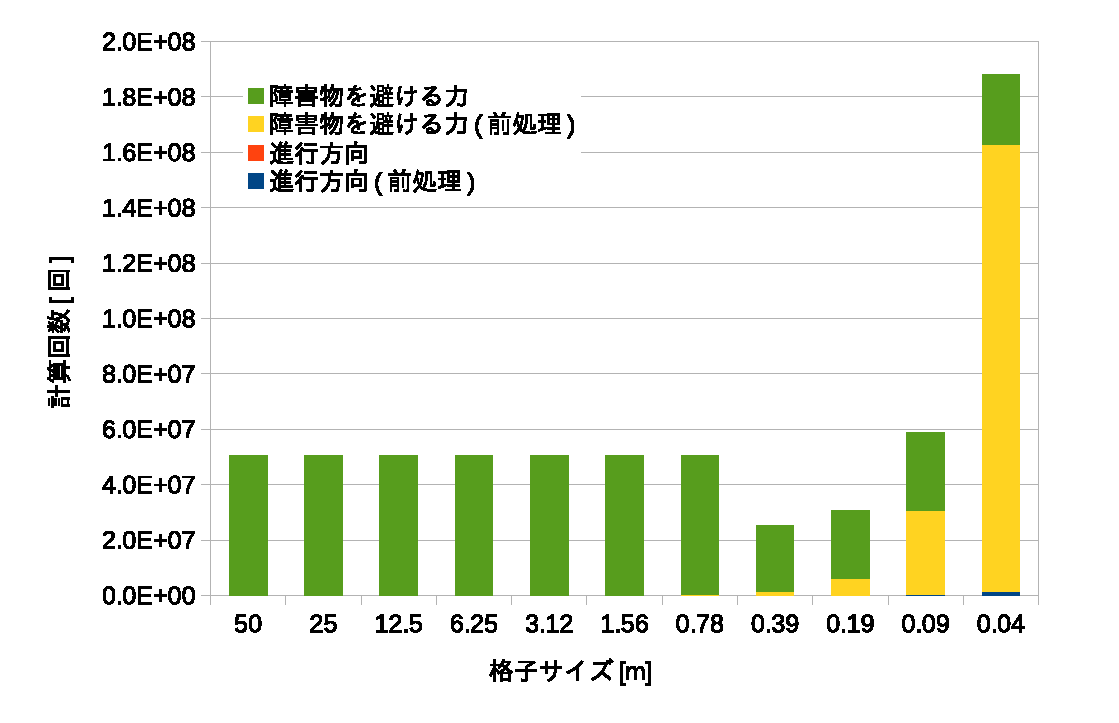
\includegraphics[width=\columnwidth]{figure/5_result_2bai_times.eps}
		\caption{通路幅2m(壁粒子2倍)の格子サイズごとの計算回数}
		\label{fig:result_2bai_times}
		\end{center}
	\end{minipage}
	\hspace{0.04\columnwidth}
	\begin{minipage}[b]{0.48\columnwidth}
		\begin{center}
		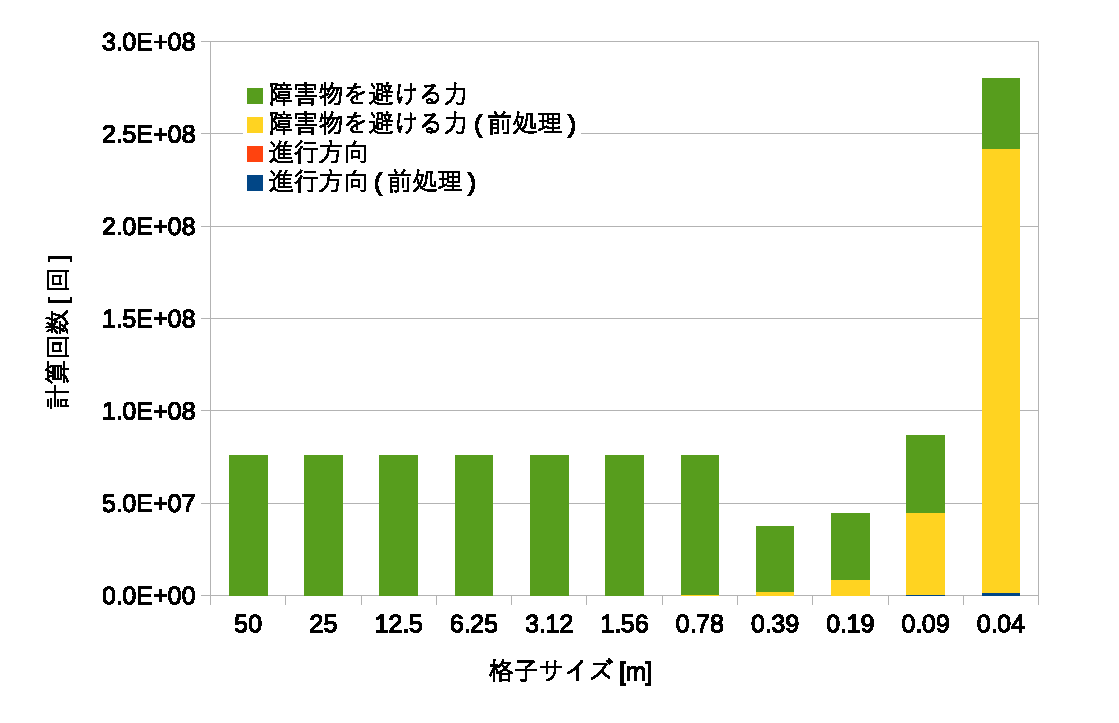
\includegraphics[width=\columnwidth]{figure/5_result_3bai_times.eps}
		\caption{通路幅2m(壁粒子3倍)の格子サイズごとの計算回数}
		\label{fig:result_3bai_times}
		\end{center}
	\end{minipage}
\end{figure}
%}}}
%昔の図{{{
%\figtb{通路幅2mの計算回数}{}{11}{5_result_2m_times.eps}{result_2m_times}
%\figtb{通路幅5mの計算回数}{}{11}{5_result_5m_times.eps}{result_5m_times}
%\figtb{通路幅10mの計算回数}{}{11}{5_result_10m_times.eps}{result_10m_times}
%\figtb{通路幅20mの計算回数}{}{11}{5_result_20m_times.eps}{result_20m_times}
%
%\figtb{通路幅2m(壁粒子2倍)の計算回数}{}{11}{5_result_2bai_times.eps}{result_2bai_times}
%\figtb{通路幅2m(壁粒子3倍)の計算回数(仮画像)}{}{11}{5_result_2bai_times.eps}{result_2bai_times}
%}}}
%削減率の表{{{
\begin{table}[tb]
  \centering
  \caption{各通路幅の格子サイズごとの計算回数の削減率[\%]}
  \label{tb:5_times_sakugenritu}
    \begin{tabular}{r|r|r|r|r}
    \hline \hline
              & 通路幅2m       & 通路幅5m       & 通路幅10m      & 通路幅20m     \\ \hline
        50.00 & 0.00           & 0.00           & 0.00           & 0.00          \\ \hline
        25.00 & 0.00           & 0.00           & 0.00           & 0.00          \\ \hline
        12.50 & 0.08           & 0.07           & 1.03           & 0.03          \\ \hline
        6.25  & 0.23           & 0.25           & -3.04          & -0.93         \\ \hline
        3.12  & 0.15           & 0.22           & -0.12          & 1.57          \\ \hline
        1.56  & 0.19           & 0.10           & 37.69          & 6.44          \\ \hline
        0.78  & 0.50           & 33.86          & \textbf{54.81} & \textbf{8.25} \\ \hline
        0.39  & \textbf{43.85} & \textbf{45.48} & 44.98          & 1.60          \\ \hline
        0.19  & 34.61          & 32.68          & 35.66          & -23.33        \\ \hline
        0.09  & -13.93         & -6.88          & -12.48         & -137.22       \\ \hline
        0.04  & -235.83        & -225.08        & -267.49        & -738.82       \\ \hline
    \end{tabular}
\end{table}
%}}}

%壁粒子数を変えたときの削減率{{{
\begin{table}[tb]
  \centering
  \caption{各通路幅の格子サイズごとの計算回数の削減率[\%]}
  \label{tb:5_bai_sakugenritu}
    \begin{tabular}{r|r|r|r}
    \hline \hline
		      & 壁粒子(1倍)    & 壁粒子(2倍)      & 壁粒子(3倍)        \\ \hline
		50.00 & 0.00           & 0.00             & 0.00               \\ \hline
		25.00 & 0.00           & 0.00             & 0.00               \\ \hline
		12.50 & 0.08           & 0.00             & 0.03               \\ \hline
		 6.25 & 0.23           & 0.03             & 0.08               \\ \hline
		 3.12 & 0.15           & 0.02             & 0.00               \\ \hline
		 1.56 & 0.19           & 0.05             & 0.11               \\ \hline
		 0.78 & 0.50           & 0.21             & 0.29               \\ \hline
		 0.39 & \textbf{43.85} & \textbf{47.00}   & \textbf{48.46}     \\ \hline
		 0.19 & 34.61          & 36.81            & 39.93              \\ \hline
		 0.09 & -13.93         & -14.68           & -13.39             \\ \hline
		 0.04 & -235.83        & -251.21          & -255.13            \\ \hline
    \end{tabular}
\end{table}
%}}}

\figref{fig:result_2bai_times},\figref{fig:result_3bai_times}より,
提案手法は,壁粒子数が増加した場合においても\figref{fig:result_2m_times}と同様に
格子サイズ0.39mから0.19mの間で削減できることが確認できる.
\figref{fig:result_2bai_times},\figref{fig:result_3bai_times}の結果から式\eqref{eq:5_sakugenritu}
を用いて算出した各配置の削減率を\tabref{tb:5_bai_sakugenritu}に示す.
\tabref{tb:5_bai_sakugenritu}中の太字の数値は,各配置の削減率の最大値を示す.
\tabref{tb:5_bai_sakugenritu}より,壁粒子数が多くなるほど,計算回数の削減率の最大値が高くなることがわかる.
これは,壁粒子の密度が高くなるほど,既存手法であるセル分割法の計算回数が増加するため,提案手法の
削減できる計算回数が多くなるためであると考えられる.

\clearpage
\subsection{シミュレーションの実行時間の測定}
\label{sec:5_calc_jikan}
\ref{sec:5_calc_times}節より,提案手法を用いることで,既存手法であるセル分割法よりも
進行方向の計算回数を削減できることが確認できた.
一方で,提案手法は,解析前にあらかじめ各格子の進行方向を計算するため,解析前の前処理の
実行時間は増加する.このため,あらかじめ計算するために必要な時間を考慮しても
格子分割を用いた進行方向の計算回数削減による高速化が有効であることを確認する.
\figref{fig:result_2m_jikan},\figref{fig:result_5m_jikan},
\figref{fig:result_10m_jikan},\figref{fig:result_20m_jikan}に通路幅ごとの
シミュレーション実行時間を,\figref{fig:5_kousokuka_haba}に式\eqref{eq:5_kousokuka}を用いて算出した
高速化率を示す.
また,\figref{fig:result_2bai_jikan},\figref{fig:result_3bai_jikan}に通路幅2mのときの
粒子数を2倍,3倍にした配置のシミュレーション実行時間を,\figref{fig:5_kousokuka_atusa}に高速化率を示す.
%
\begin{align}
	\mbox{高速化率[倍]} = \frac{\mbox{セル分割法の実行時間[s]}}
    {\mbox{提案手法の実行時間[s]}}
    \label{eq:5_kousokuka}
\end{align}
%
\figref{fig:result_2m_jikan},\figref{fig:result_5m_jikan},
\figref{fig:result_10m_jikan},\figref{fig:result_20m_jikan},
\figref{fig:5_kousokuka_haba}より,
提案手法は,セル分割法よりも最大△△倍高速であり,
従来手法よりも解析時間が最大○○割削減できることが確認できる.
また,格子サイズが小さくなるほど,前処理の計算にかかる時間の
割合が多くなり,通路幅2mでは0.09m,通路幅5mでは0.09m,通路幅10mでは
0.19m,通路幅20mでは0.39m以下の格子サイズで,従来手法よりも
遅くなることが確認できる.
前処理時間にかかる時間は,\ref{sec:5_calc_times}節で示した
前処理中の計算回数が占める割合の傾向と同様であることがわかる.
従来手法よりも高速に解析できる提案手法の格子サイズは,
通路幅2mで0.39mから0.19m,
通路幅5mで0.78mから0.19m,
通路幅10mで1.56mから0.19m,
通路幅20mで6.25mから0.39mであり,
通路幅が広くなるほど,従来手法よりも高速に解析できる格子サイズが
多くなることがわかる.
これをふまえると,従来手法よりも高速に解析できる提案手法の
格子サイズは,エージェントが通る場所の障害物と障害物の間の距離に
応じて変わることが考えられる.
\textbf{[壁粒子数を変えた時のシミュレーション実行時間と高速化率
について述べる!!!]} 

\figref{fig:result_2bai_jikan},\figref{fig:result_3bai_jikan},
\figref{fig:5_kousokuka_atusa}より,
提案手法のセル分割法に対する高速化率は,
壁粒子数1倍のときで最大○○倍,
壁粒子数2倍のときで最大○○倍,
壁粒子数3倍のときで最大○○倍であり,
壁粒子数が増えるほど高速化率の最大値が高くなることが確認できる.
これは,壁粒子を増やす方法が壁粒子の密度が高くなるような設定をしているため,
密度が高くなるほど,\ref{sec:5_calc_times}節で示した計算回数が削減でき,
解析時間の短縮に繋がったと考えられる.



\begin{figure}[tb]
	\begin{minipage}[b]{0.48\columnwidth}
		\begin{center}
		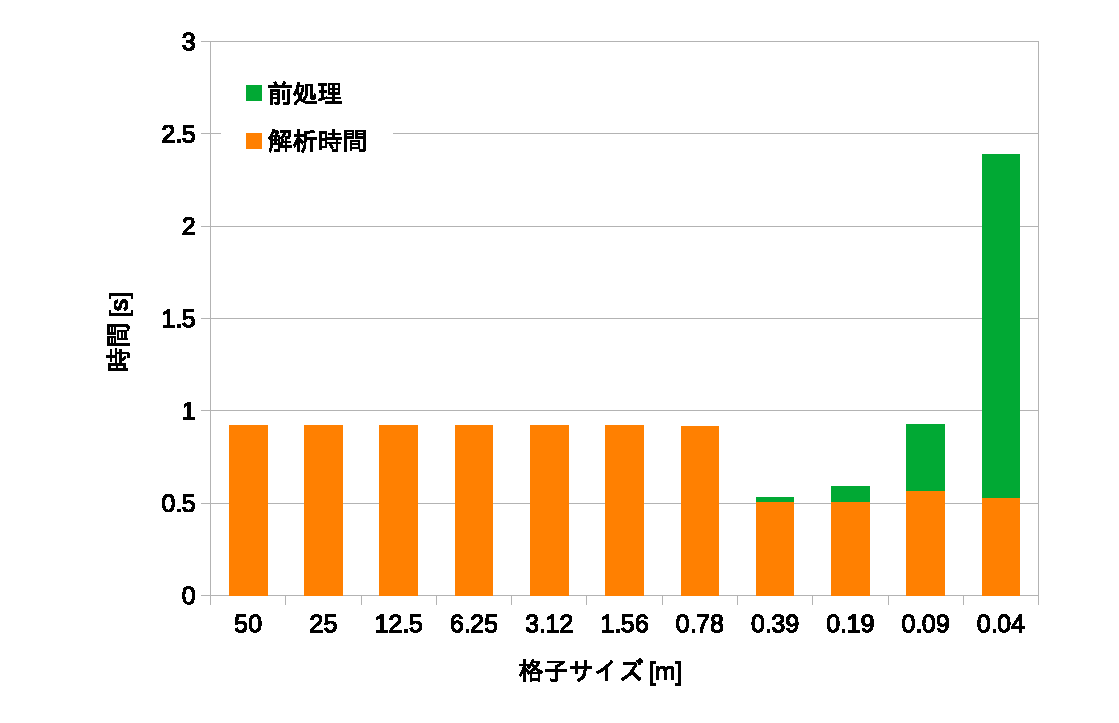
\includegraphics[width=\columnwidth]{figure/5_2m_jikan.eps}
		\caption{通路幅2mの格子サイズごとの解析時間}
		\label{fig:result_2m_jikan}
		\end{center}
	\end{minipage}
	\hspace{0.04\columnwidth}
	\begin{minipage}[b]{0.48\columnwidth}
		\begin{center}
		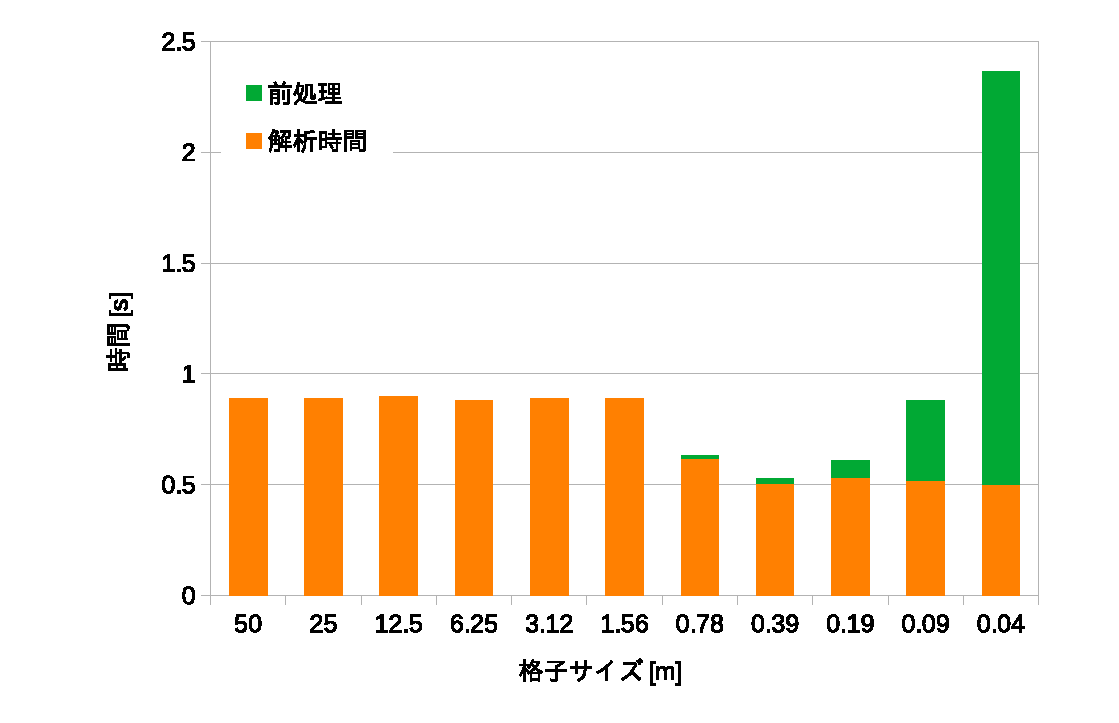
\includegraphics[width=\columnwidth]{figure/5_5m_jikan.eps}
		\caption{通路幅5mの格子サイズごとの解析時間}
		\label{fig:result_5m_jikan}
		\end{center}
	\end{minipage}
\end{figure}

\begin{figure}[tb]
	\begin{minipage}[b]{0.48\columnwidth}
		\begin{center}
		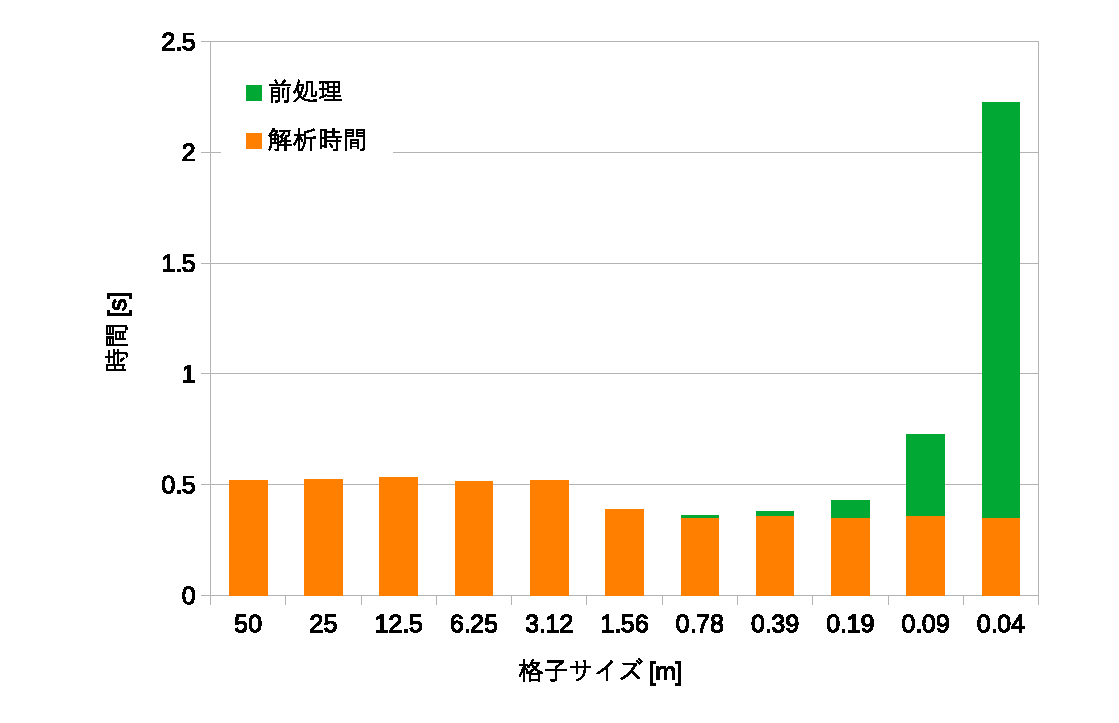
\includegraphics[width=\columnwidth]{figure/5_10m_jikan.eps}
		\caption{通路幅10mの格子サイズごとの解析時間}
		\label{fig:result_10m_jikan}
		\end{center}
	\end{minipage}
	\hspace{0.04\columnwidth}
	\begin{minipage}[b]{0.48\columnwidth}
		\begin{center}
		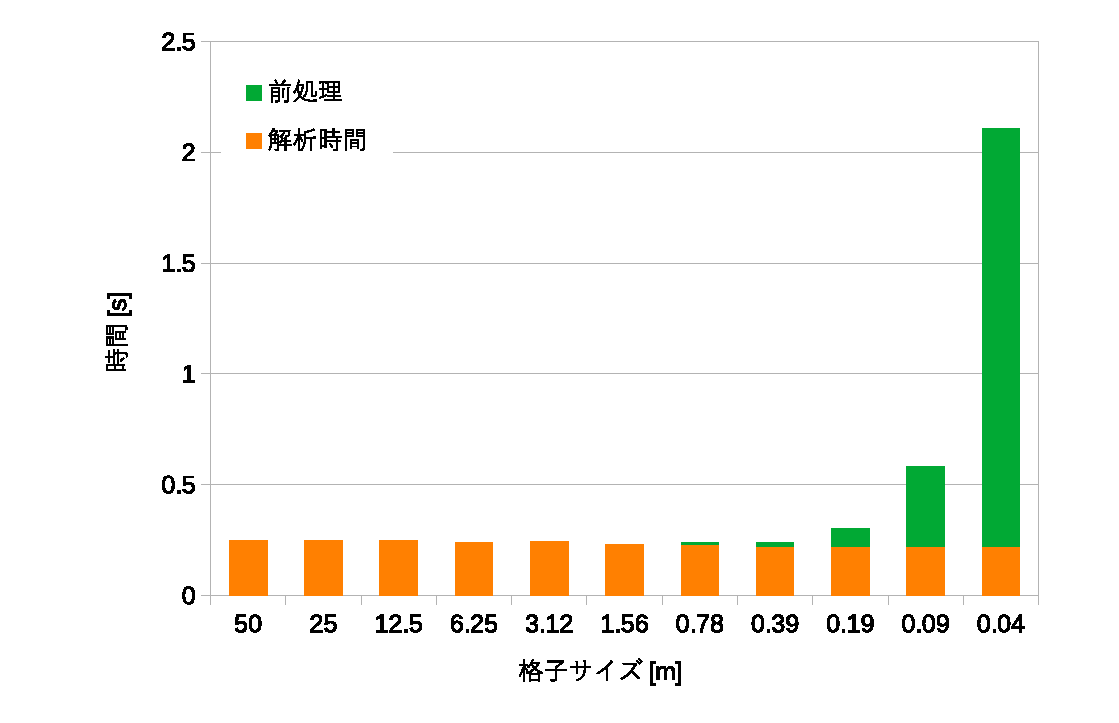
\includegraphics[width=\columnwidth]{figure/5_20m_jikan.eps}
		\caption{通路幅20mの格子サイズごとの解析時間}
		\label{fig:result_20m_jikan}
		\end{center}
	\end{minipage}
\end{figure}

\begin{figure}[tb]
	\begin{minipage}[b]{0.48\columnwidth}
		\begin{center}
		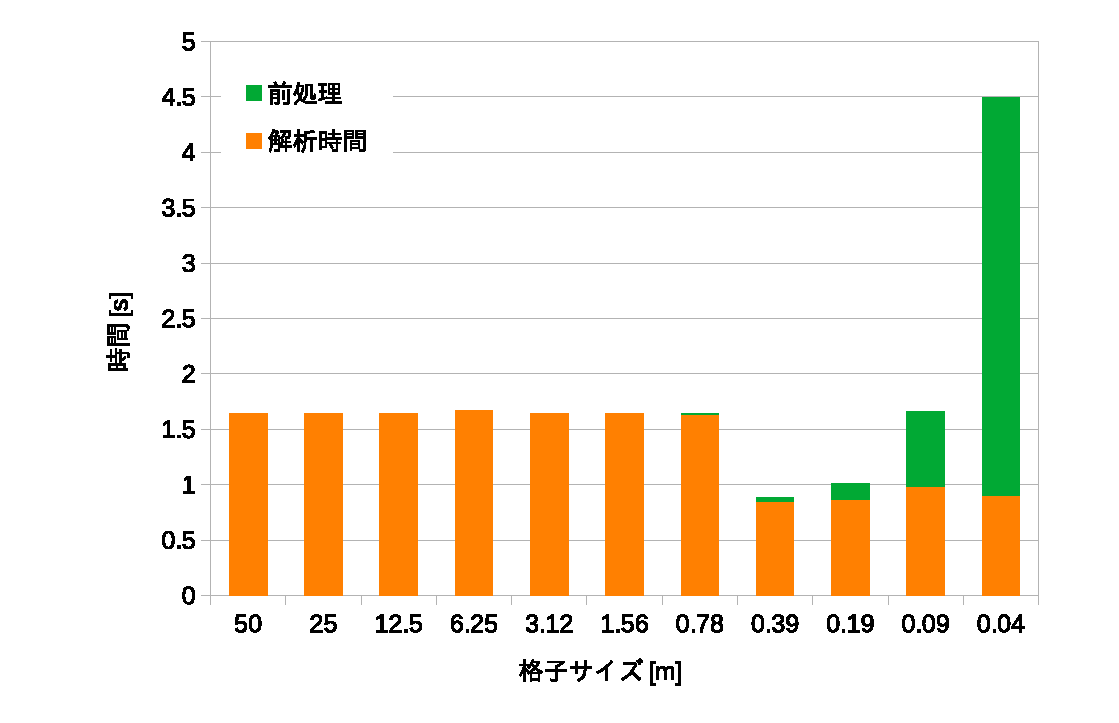
\includegraphics[width=\columnwidth]{figure/5_2bai_jikan.eps}
		\caption{通路幅2m(粒子数2倍)の格子サイズごとの解析時間}
		\label{fig:result_2bai_jikan}
		\end{center}
	\end{minipage}
	\hspace{0.04\columnwidth}
	\begin{minipage}[b]{0.48\columnwidth}
		\begin{center}
		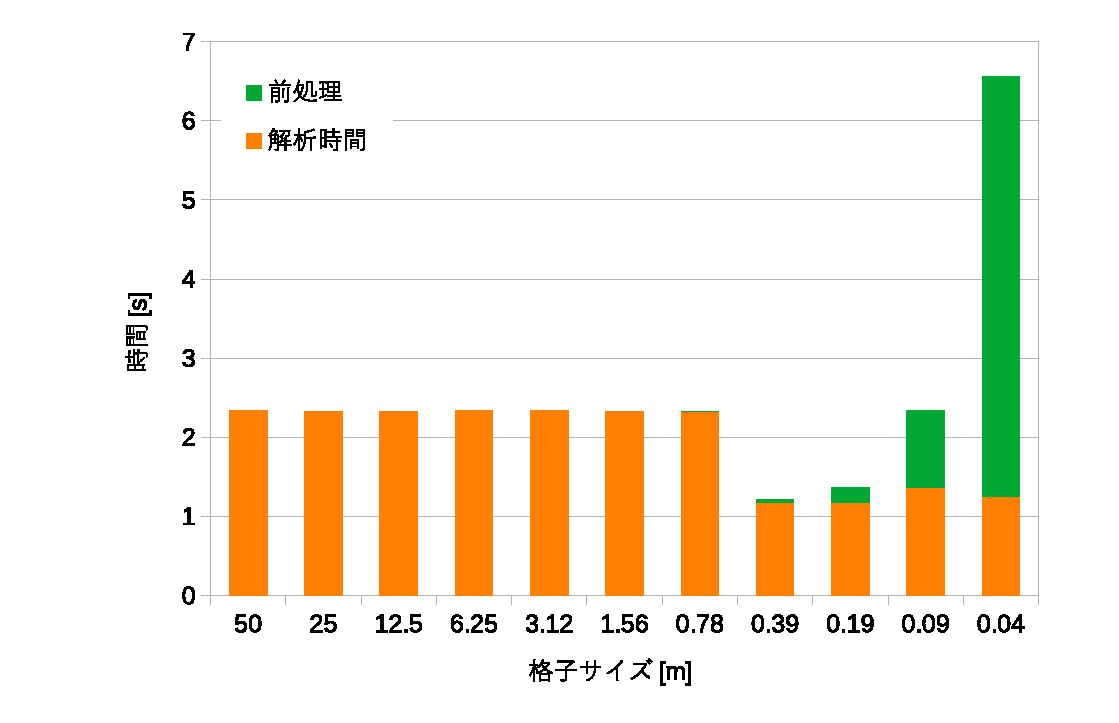
\includegraphics[width=\columnwidth]{figure/5_3bai_jikan.eps}
		\caption{通路幅3m(粒子数3倍)の格子サイズごとの解析時間}
		\label{fig:result_3bai_jikan}
		\end{center}
	\end{minipage}
\end{figure}


\begin{figure}[tb]
 \begin{center}
  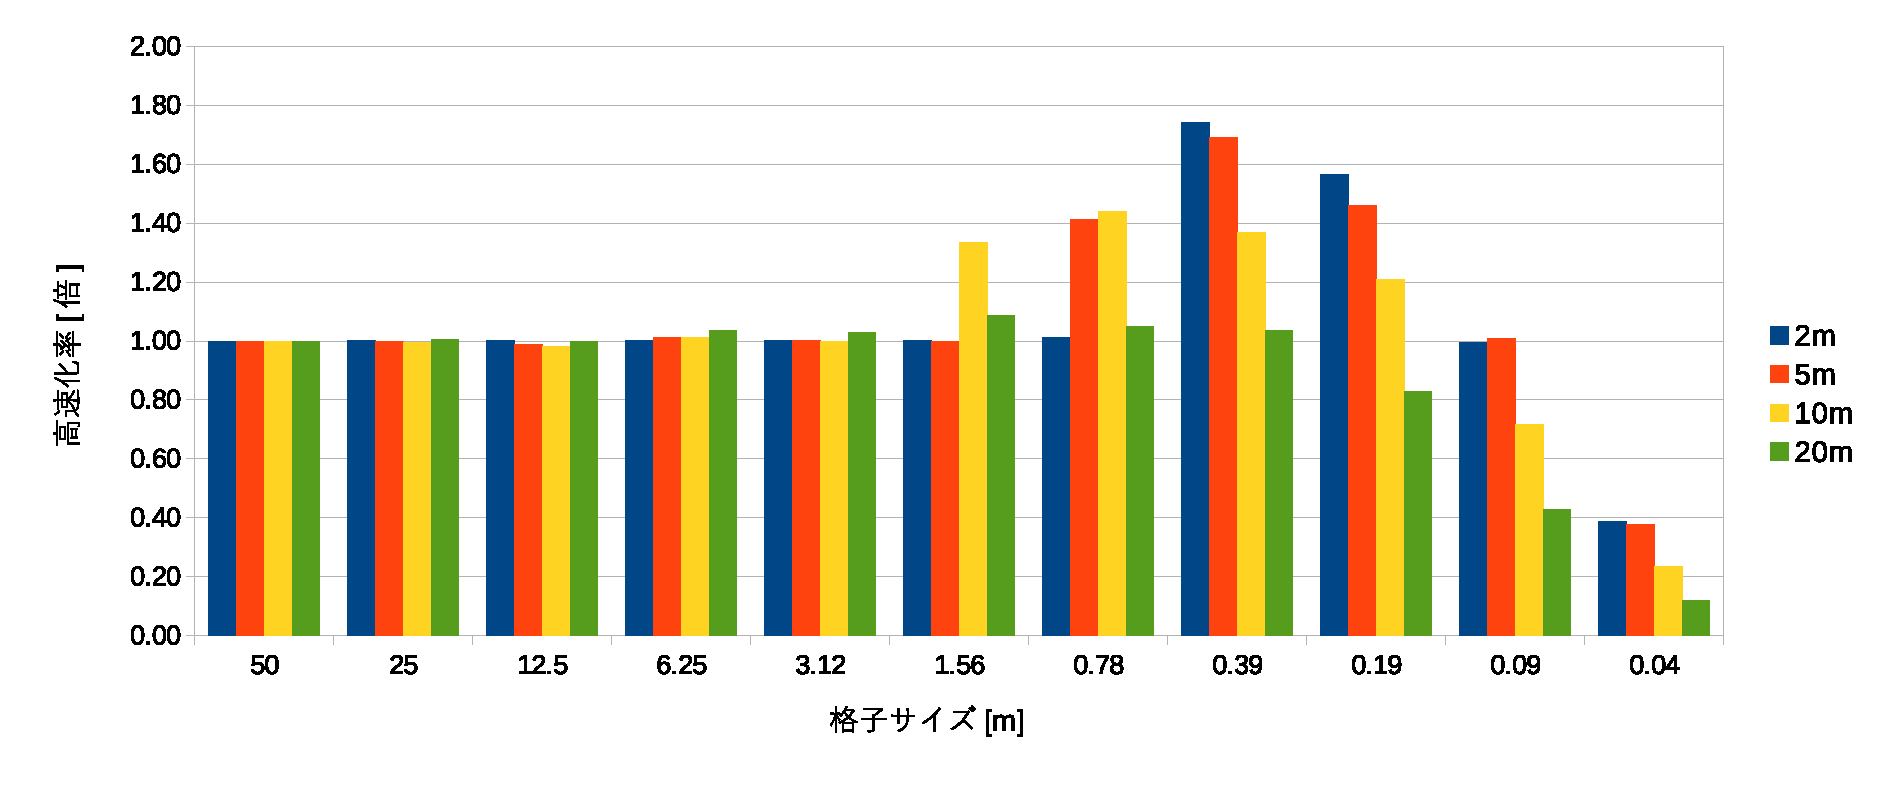
\includegraphics[width=12.5cm,clip]{figure/5_kousokukaritu.eps}
  \caption{通路幅を変えたときの高速化率}
  \label{fig:5_kousokuka_haba}
 \end{center}
\end{figure}


\begin{figure}[tb]
 \begin{center}
  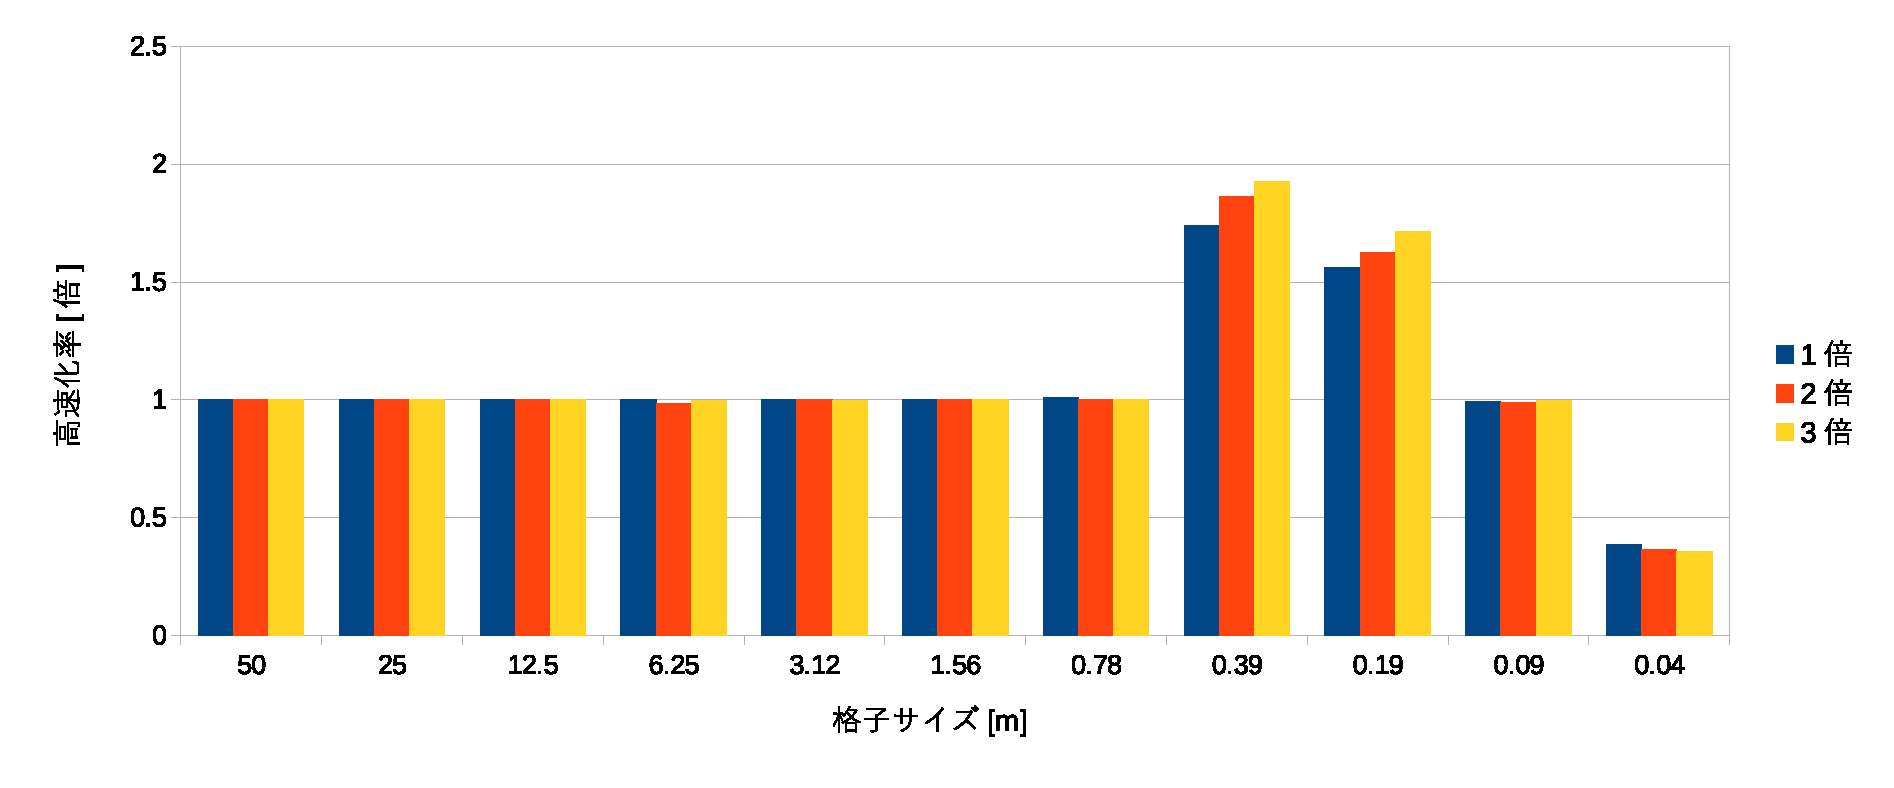
\includegraphics[width=12.5cm,clip]{figure/5_bai_kousokukaritu.eps}
  \caption{壁粒子数を変えたときの高速化率}
  \label{fig:5_kousokuka_atusa}
 \end{center}
\end{figure}


\clearpage
\subsection{シミュレーション精度の測定}
\ref{sec:5_calc_jikan}節より,
提案手法は,一部の格子サイズでセル分割法よりも高速に解析できることが確認できた.
一方で,本手法は,解析領域を格子状に分割した格子ごとに計算した進行方向ベクトル$e$と
障害物を避ける力$F_{iW}$を解析中に用いるため,セル分割法のシミュレーションと比べて
シミュレーション誤差が生じる手法となる.
このため,提案手法の格子ごとのシミュレーション結果と従来手法であるセル分割法の
シミュレーション結果を比較し,シミュレーション精度を確かめる.
誤差は,提案手法とセル分割法が算出した時間ステップごとに各エージェントの座標を
出力し,2手法の同時刻・同エージェントどうしによるエージェント間距離の最大値とする.
\textbf{
[図○○に各配置のシミュレーションの最大誤差を示す.]
}


\clearpage
\subsection{避難シミュレーションに対する提案手法の有効性}
\label{sec:5_real}
本節では,実問題に対する提案手法の有効性を示すために,実際の状況下で
避難シミュレーションを行い,シミュレーション実行時間とシミュレーション精度を
確かめる.
本評価に用いるエージェントの初期配置は,\figref{fig:kyositu_haichi},\figref{fig:pc_haichi}に示すように,大学の演習室や教室の避難時の配置で設定する.
\figref{fig:kyositu_haichi},\figref{fig:pc_haichi}の黒点は壁粒子,紫色の点はエージェント,青色の丸は経由地の座標およびゴール判定の大きさ,赤色の矢印は経由地のグラフを示す.
それぞれの配置のエージェントや壁,経由地は,\tabref{tb:haichi_para}に示すような数で配置する.
本測定では,パラメータを\tabref{tb:result_para}で設定し,すべてのエージェントが
部屋から避難できるまでを刻み値0.001で解析する.
\textbf{
[結果を表示する]
}


\begin{eqnarray}
\label{eq:gosa_hinan}
\mbox{誤差$[\%]$} = \left | \frac{C_{time} - T_{time}}{C_{time}} \right | \times 100
\end{eqnarray}

\begin{figure}[tb]
	\begin{minipage}[b]{0.5\columnwidth}
		\centering
		\includegraphics[width=\columnwidth]{figure/kyositu_v2.eps}
		\caption{教室の初期配置}
    \label{fig:kyositu_haichi}
	\end{minipage}
	\begin{minipage}[b]{0.5\columnwidth}
		\centering
		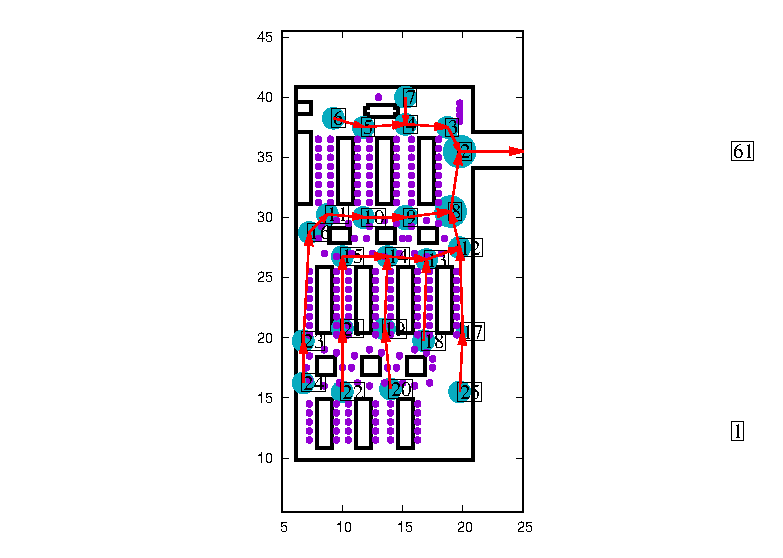
\includegraphics[width=\columnwidth]{figure/pc_m.eps}
		\caption{演習室の初期配置}
    \label{fig:pc_haichi}
	\end{minipage}
\end{figure}



\begin{table}[tb]
  \begin{center}
    \caption{各配置の詳細}
    \label{tb:haichi_para}
    \begin{tabular}{c|c|c}
      \hline \hline
      & 教室 & 演習室 \\ \hline 
      エージェント数[人] & 96 & 204 \\ \hline
      壁粒子数[個] & 1037 & 1454\\ \hline
      経由地数[個] & 12   & 26 \\ \hline
      解析領域 & $50m\times50m$ & $50m\times50m$ \\ \hline
    \end{tabular}
  \end{center}
\end{table}


%教室と演習室の解析時間{{{
\begin{figure}[tb]
	\begin{minipage}[b]{0.48\columnwidth}
		\begin{center}
		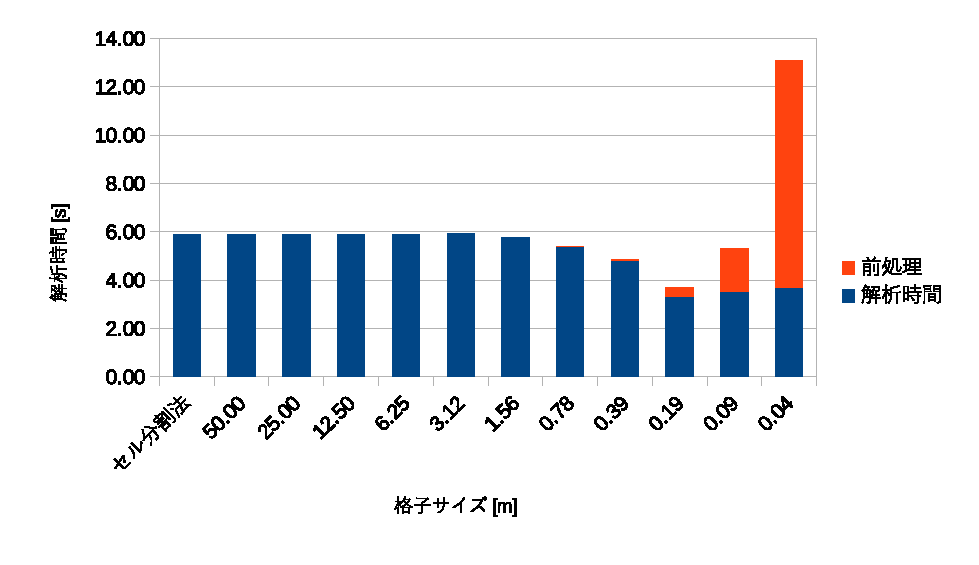
\includegraphics[width=\columnwidth]{figure/20231016_kyositu_time.eps}
		\caption{教室の配置における格子サイズごとの解析時間}
		\label{fig:kyositu_time}
		\end{center}
	\end{minipage}
	\hspace{0.04\columnwidth}
	\begin{minipage}[b]{0.48\columnwidth}
		\begin{center}
		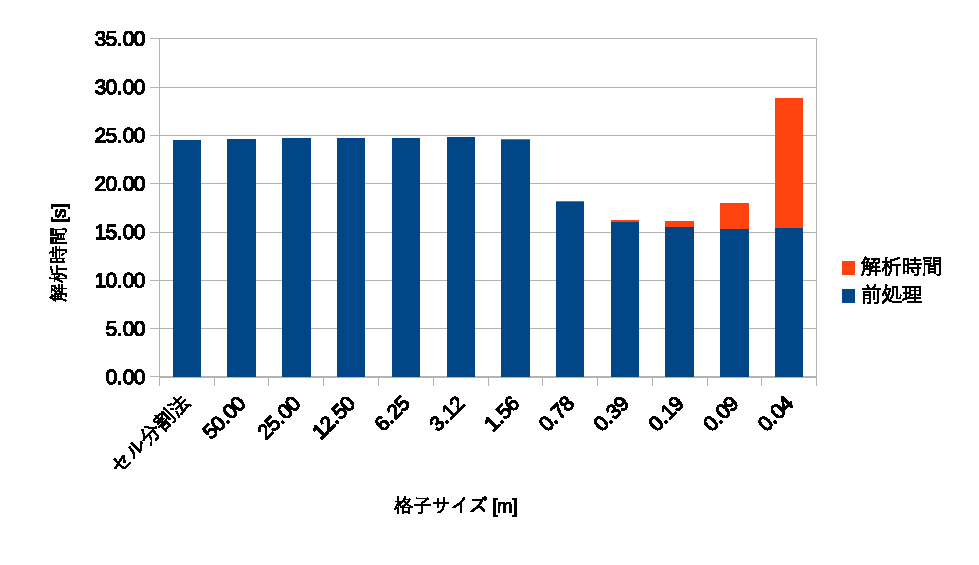
\includegraphics[width=\columnwidth]{figure/20231016_pc_time.eps}
		\caption{演習室の配置における格子サイズごとの解析時間}
		\label{fig:pc_time}
		\end{center}
	\end{minipage}
\end{figure}
%}}}

%教室と演習室の誤差{{{
\begin{figure}[tb]
	\begin{minipage}[b]{0.48\columnwidth}
		\begin{center}
		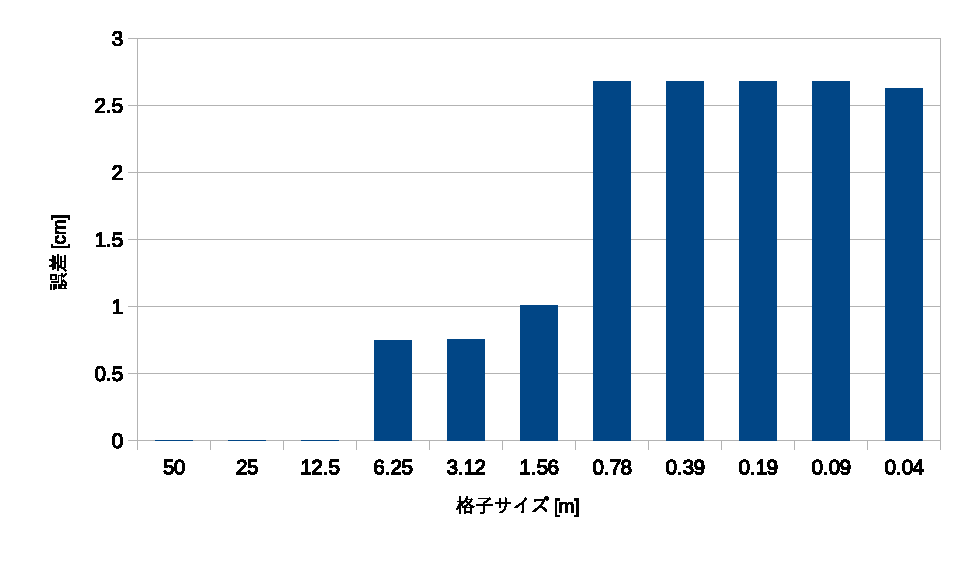
\includegraphics[width=\columnwidth]{figure/20231016_kyositu_gosa.eps}
		\caption{教室の配置における格子サイズごとの最大誤差}
		\label{fig:kyositu_gosa}
		\end{center}
	\end{minipage}
	\hspace{0.04\columnwidth}
	\begin{minipage}[b]{0.48\columnwidth}
		\begin{center}
		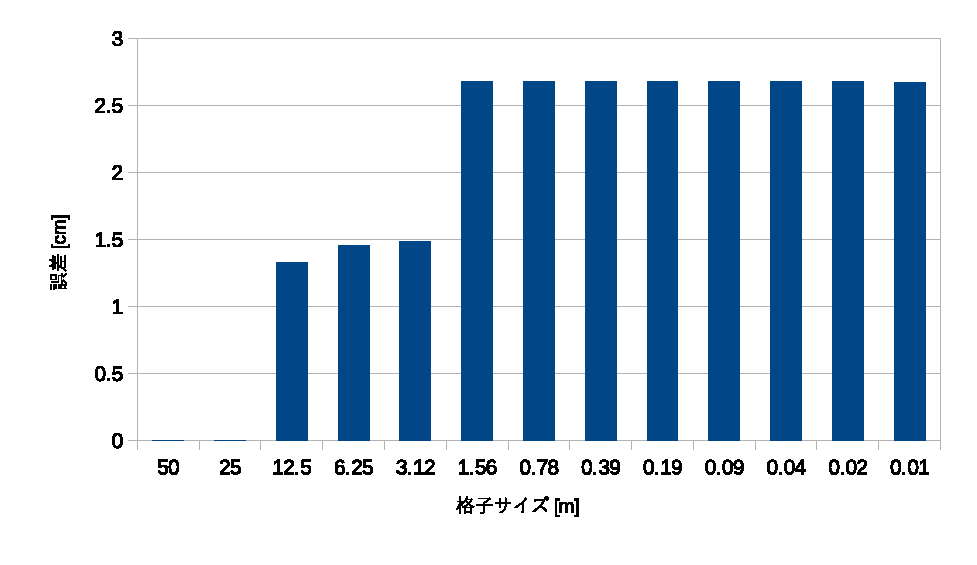
\includegraphics[width=\columnwidth]{figure/20231016_pc_gosa.eps}
		\caption{演習室の配置における格子サイズごとの最大誤差}
		\label{fig:pc_gosa}
		\end{center}
	\end{minipage}
\end{figure}
%}}}


%\figtb{格子サイズごとの解析時間(教室)}{}{8.0}{20231016_kyositu_time}{kyositu_time}
%\figtb{格子サイズごとの解析時間(演習室)}{}{8}{20231016_pc_time.eps}{pc_time}
%\figtb{格子サイズごとの最大誤差(教室)}{}{8.0}{20231016_kyositu_gosa}{kyositu_gosa}
%\figtb{格子サイズごとの最大誤差(演習室)}{}{8}{20231016_pc_gosa.eps}{kyositu_gosa}


\clearpage
\section{本章のまとめ(工事中)}
工事中.
